\documentclass{article}
\usepackage[utf8]{inputenc}
\usepackage{graphicx}
\usepackage{multirow}
\usepackage{subcaption}

\usepackage{lipsum}
\usepackage{listings}
\usepackage{xcolor}

\usepackage{mathtools}
\usepackage{xcolor}
\usepackage{listings}

\newcommand{\divider}{\par\noindent\rule{0.9375\textwidth}{0.4pt}}

\newcommand{\DeclareAutoPairedDelimiter}[3]{%
  \expandafter\DeclarePairedDelimiter\csname Auto\string#1\endcsname{#2}{#3}%
  \begingroup\edef\x{\endgroup
    \noexpand\DeclareRobustCommand{\noexpand#1}{%
      \expandafter\noexpand\csname Auto\string#1\endcsname*}}%
  \x}

\DeclareAutoPairedDelimiter{\tuple}{\langle}{\rangle}
\DeclareAutoPairedDelimiter{\array}{[}{]}
\DeclareAutoPairedDelimiter{\ceil}{\lceil}{\rceil}
\DeclareAutoPairedDelimiter{\floor}{\lfloor}{\rfloor}



\newcommand{\answer}[1]{{\color{violet}%
        #1
    }%
}

\newcommand{\finalanswer}[1]{
    \noindent\color{red}\fbox{%
        \parbox{0.975\linewidth}{\color{violet}%
            #1
        }%
    }
}

% Default fixed font does not support bold face
\DeclareFixedFont{\ttb}{T1}{txtt}{bx}{n}{10} % for bold
\DeclareFixedFont{\ttm}{T1}{txtt}{m}{n}{10}  % for normal

% custom colors for lst
\definecolor{deepblue}{rgb}{0,0,0.5}
\definecolor{deepred}{rgb}{0.6,0,0}
\definecolor{deepgreen}{rgb}{0,0.5,0}

% Python style for highlighting
\newcommand\pythonstyle{\lstset{
language=Python,
basicstyle=\ttm,
morekeywords={self},              % Add keywords here
keywordstyle=\ttb\color{deepblue},
emph={MyClass,__init__},          % Custom highlighting
emphstyle=\ttb\color{deepred},    % Custom highlighting style
stringstyle=\color{deepgreen},
frame=tb,                         % Any extra options here
showstringspaces=false,
}}

% Python environment
\lstnewenvironment{python}[1][]
{
\pythonstyle
\lstset{#1}
}
{}

\newcommand\cppstyle{\lstset{
    language=C++, % choose the language of the code
    basicstyle=\fontfamily{pcr}\selectfont\footnotesize\color{black},
    keywordstyle=\color{black}\bfseries, % style for keywords
    numbers=left, % where to put the line-numbers
    numberstyle=\scriptsize, % the size of the fonts that are used for the 
    showspaces=false, % show spaces adding particular underscores
    showstringspaces=false, % underline spaces within strings
    showtabs=false, % show tabs within strings adding particular underscores
    frame=single, % adds a frame around the code
    tabsize=2, % sets default tabsize to 2 spaces
    rulesepcolor=\color{gray},
    rulecolor=\color{black},
    captionpos=b, % sets the caption-position to bottom
    breaklines=true, % sets automatic line breaking
    breakatwhitespace=false, 
    numbersep=6pt,
}}

% C++ environment
\lstnewenvironment{c++}[1][]
{
\cppstyle
\lstset{#1}
}
{}

\newcommand{\hb}{\ensuremath{\longrightarrow}\xspace}
\newcommand{\chb}{\ensuremath{\|}}

\newenvironment{warning}
  {\par\begin{mdframed}[linewidth=2pt,linecolor=red,backgroundcolor=yellow,frametitle=Warning]%
    \begin{list}{}{\leftmargin=1cm
                  \labelwidth=\leftmargin}\item[\Large\ding{43}]}
  {\end{list}\end{mdframed}\par}


\title{CMSE 822 Final Project }
\author{Carolyn Wendeln $\&$ Gabe Appleton}

\date{December 13, 2021}

\begin{document}

\maketitle

\section{Introduction}

Modern  astrophysical  research  has  become  increasingly  dominated  by  large-scale, multi-dimensional simulations. Phenomena such as supernovae core collapse, coronal mass ejections, or neutron star mergers all rely on such multi-scale simulations. A common theme throughout the hardest of these simulations is the tight coupling of the different underlying physical phenomena involved over broad scales in both length and time. Although these multi-scale simulations have become a necessity to increasing our knowledge, they often require an ever-increasing amount of computational resources.

One key feature that most of these astrophysical phenomena have in common is that they are often coupled to nonlinear hyperbolic partial differential equations (PDEs).
Equations such as Euler, Cauchy, or Navier–Stokes are often used for simulating astrophysical plasmas. The Simulation of these equations often calls for techniques such as adaptive mesh refinement (AMR), high order finite difference, or high order finite volume methods.

For this research project, we will be investigating second and fourth order discretization of hyperbolic PDEs. In particular, we will look at the two dimensional form of the Advection Equation, Inviscid Burgers' Equation, and Viscous Burgers' Equation. We chose these equations because they are generally easier to solve compared to Euler, Cauchy, and Navier-Stokes. 
This work will focus on these three equations over a periodic domain on a uniform mesh grid using finite difference methods.

The goal of this research project is to understand the underlying issues surrounding hyperbolic solvers for fluid equations. We will investigate various optimization techniques for a single node. Our work will begin with parallelization using \texttt{OpenMP} to target CPUs. After parallelisation, we will employ other techniques such as cache blocking and loop scheduling to see the effects of strong and weak scaling.


\section{Methodology}
\subsection{Finite Difference Methods for Hyperbolic PDEs}
For this research project, we look to solve and parallelize three PDEs commonly used for simulating fluid dynamics. The first is the linear Advection Equation. This equation can be described as follows: 

\begin{equation}
 \frac{\partial a}{\partial t} + u \frac{\partial a}{\partial x} = 0
\end{equation}

where $a(x,t)$ is a scalar quantity for a fluid and $u$ is the velocity at which it is advected. For our research project, we chose to make $a(x,t)$ a Gaussian function of the form: 

\begin{equation}
a(x,t) = a_0(t) e^{- 50 (x - 0.5)^2 }
\end{equation}

To solve this PDE, we use a finite-difference discretization. For this method, the spatial domain is divided into a sequence of points where the solution of $a(x,t)$ is stored. The PDE is then solved numerically by discretizing the solution at these points. Figure \ref{Finite_Difference_Grid} shows a representation of the discretized grid.
Let the index $i$ denote the point's location, and $a_i$ denote the discrete value of $a(x)$ at point $i$. To discretize in time, we denote the time-level with a superscript $n$, such that $a_i^n = a(x_i, t_n)$. For a fixed $\Delta t$, a time level $n$ corresponds to a time of $t = n \Delta t$. A first-order accurate discretization centered around the point $i$ is then given as:


\begin{figure}[b]
\centering
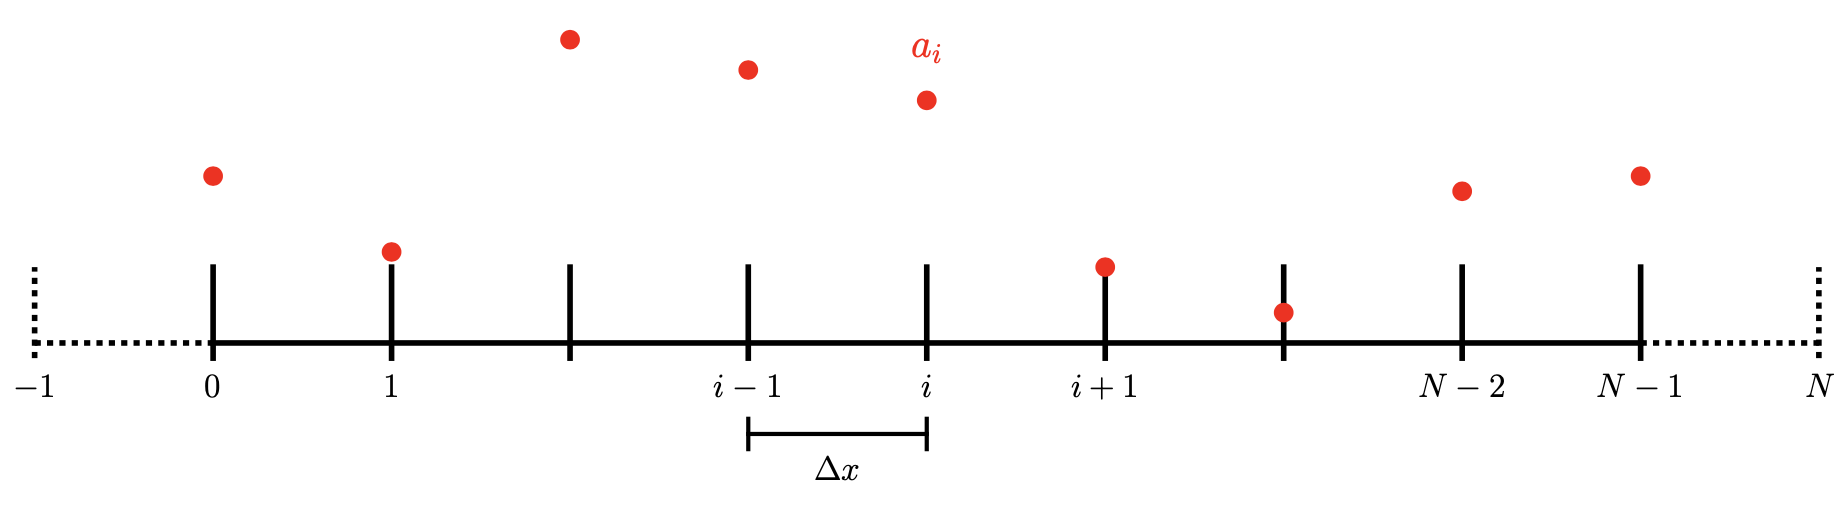
\includegraphics[width=1.0\textwidth]{Images/Finite_Difference_Grid.png}
\caption{A simple finite-difference grid \cite{zingale_2020}. The solution is stored at each of the labeled points. The dotted lines show the ghost points used to extend our grid past the physical boundaries to accommodate boundary conditions. In this instance, we assume a periodic domain, so the points $0$ and $N-1$ are the same physical point in space.}
\label{Finite_Difference_Grid}
\end{figure}


\begin{equation}
 \frac{a_i^{n+1} - a_i^n}{\Delta t} + u \frac{a_{i+1}^n - a_{i-1}^n}{2 \Delta x}  = 0
\end{equation}

This is a forward-time, centered-space explicit method, since the new solution, $a_i^{n+1}$, depends only on information at the old time level $n$. When implemented into \texttt{C++}, we are iterating through time steps $n$ and displacement steps $i$ (i.e., $a_i^n$) to solve for $a_i^{n+1}$.




The second equation we wish to investigate is the Inviscid Burgers’ Equation. This equation is a nonlinear hyperbolic equation, and is given as:

\begin{equation}
 \frac{\partial a}{\partial t} + a \frac{\partial a}{\partial x} = 0
\end{equation}

Here $a(x,t)$ is both the quantity being advected and the speed at which it is moving. The centered-difference discretization for the Inviscid Burgers' Equation is then:

\begin{equation}
 \frac{a_i^{n+1} - a_i^n}{\Delta t} +  a_i^n ( \frac{a_{i+1}^n - a_{i-1}^n}{2 \Delta x} ) = 0
\end{equation}

The third and final equation we wish to investigate is the Viscous Burgers' Equation. This equation is written as such:

\begin{equation}
 \frac{\partial a}{\partial t} + a \frac{\partial a}{\partial x} = \nu \frac{\partial ^2 a}{\partial x^2} 
\end{equation}

Here $\nu$ is the viscosity. The centered-difference discretization for the Viscous Burgers' Equation is then:

\begin{equation}
 \frac{a_i^{n+1} - a_i^n}{\Delta t} + a_i^n ( \frac{a_{i+1}^n - a_{i-1}^n}{2 \Delta x} ) = \nu (\frac{a_{i+1}^n - 2a_i^n - a_{i-1}^n}{{\Delta x}^2})
\end{equation}


 A visual representation of the Viscous Burgers Equation can be seen in Figure \ref{2D_Vis_Burg_Vis}. For this visualization, our x and y domain is between the values of 0 and 1 on a $512 \times 512$ grid. The centered-difference discretization for the Viscous Burgers' Equation was used to solve up to $t$ = 0.3 seconds for $n = 1,000$ time steps. A time of $t = 0.3$ was chosen to prevent the formation of a shock. 

\begin{figure}[h]
\begin{subfigure}{.5\textwidth}
  \centering
  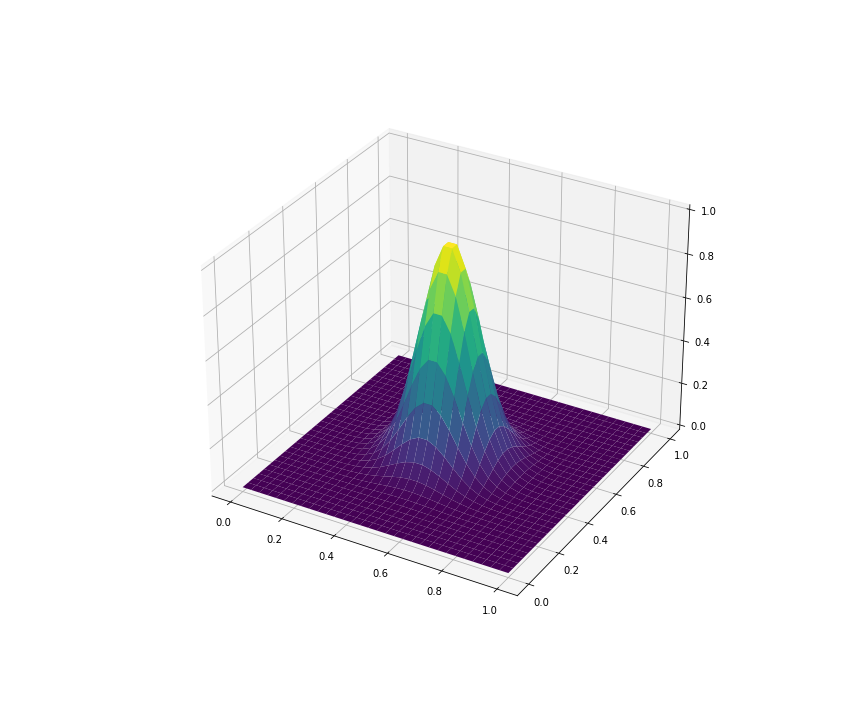
\includegraphics[width=1.0\linewidth]{Images/2D_Viscous_Burgers_Graph_0.png}
  \caption{Time step $n$ = 0}
  \label{fig:sfig1}
\end{subfigure}%
\begin{subfigure}{.5\textwidth}
  \centering
  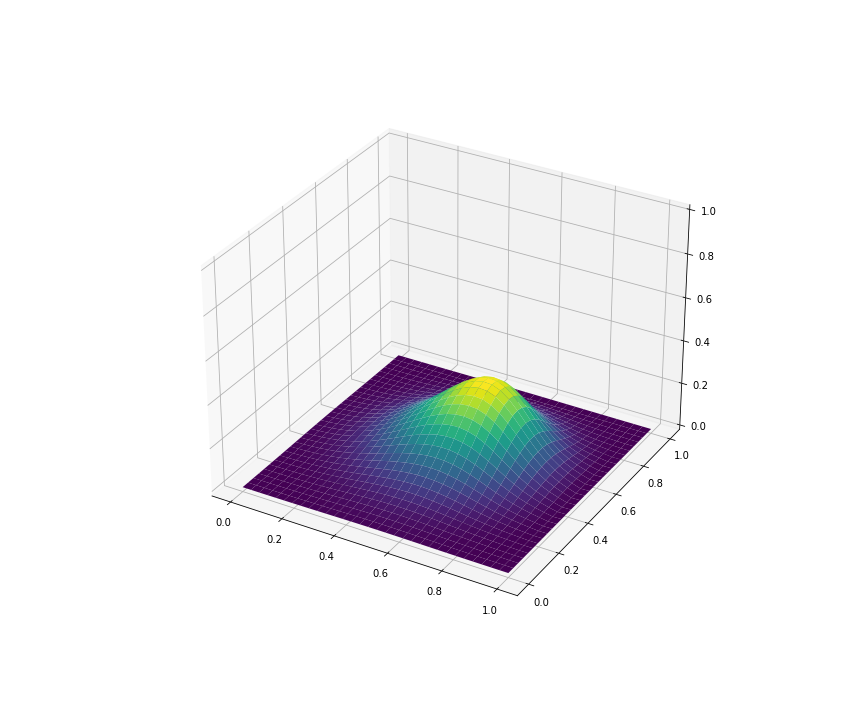
\includegraphics[width=1.0\linewidth]{Images/2D_Viscous_Burgers_Graph_999.png}
  \caption{Time step $n$ = 1000}
  \label{fig:sfig2}
\end{subfigure}
\caption{Visualization of the 2D Viscous Burgers' Equation}
\label{2D_Vis_Burg_Vis}
\end{figure}


\subsection{Parallization Techniques}
For this research project we aim to parallize our code using \texttt{OpenMP}. Our main interest is speeding up the major loop which iterates through the bulk of our spatial domain. The boundaries of our domain are not included in this loop, as they have specific boundary conditions that must be met to maintain periodicity. As an example, the major loop of our 1D Advection code is as follows:

\begin{c++}
for(int t=0; t<n; ++t)  {
    double start = omp_get_wtime();

    #pragma omp parallel for num_threads(thrd_cnt)
    for(int i=1; i<(N-2); ++i)  {
        a_write[i] = a_read[i] - 
        (((u * delta_t) / (2 * delta_x))*(a_read[i+1] - a_read[i-1]));
    }
    	
    loop_time[t] = omp_get_wtime() - start;
}	
\end{c++}



In addition to parallelizing our code using \texttt{\#pragma omp parallel}, we are interested in seeing the effect on computation time if we use a loop scheduler. Loop schedulers are a helpful way to assign loop iterations to the number of threads available. The three types of loop schedulers we are interested in for this study are static, dynamic, and guided. 

The static scheduler assigns a consecutive block of iterations to each thread. If a run has $t$ threads, each thread will be assigned $\tfrac{1}{t}$ of the iterations. Static allows for a user specified chunk size for the size of blocks. If all iterations take roughly the same amount of time, static may be the most efficient loop scheduler.
 
 The dynamic scheduler assigns blocks of iterations via a task queue, where threads will take a chunk of these tasks whenever it finishes with its previous tasks. Similar to static, dynamic allows for a specified chunk size. Dynamic is most helpful when iterations will take a variable amount of time to execute.
 
 Lastly, the guided scheduler gradually decreases the chunk size. It does so under the assumption that large chunks carry the least overhead, but smaller chunks are better for load balancing. The various schedules are illustrated in Figure \ref{Loop_Schedule}.
 
\begin{figure}[h]
\centering
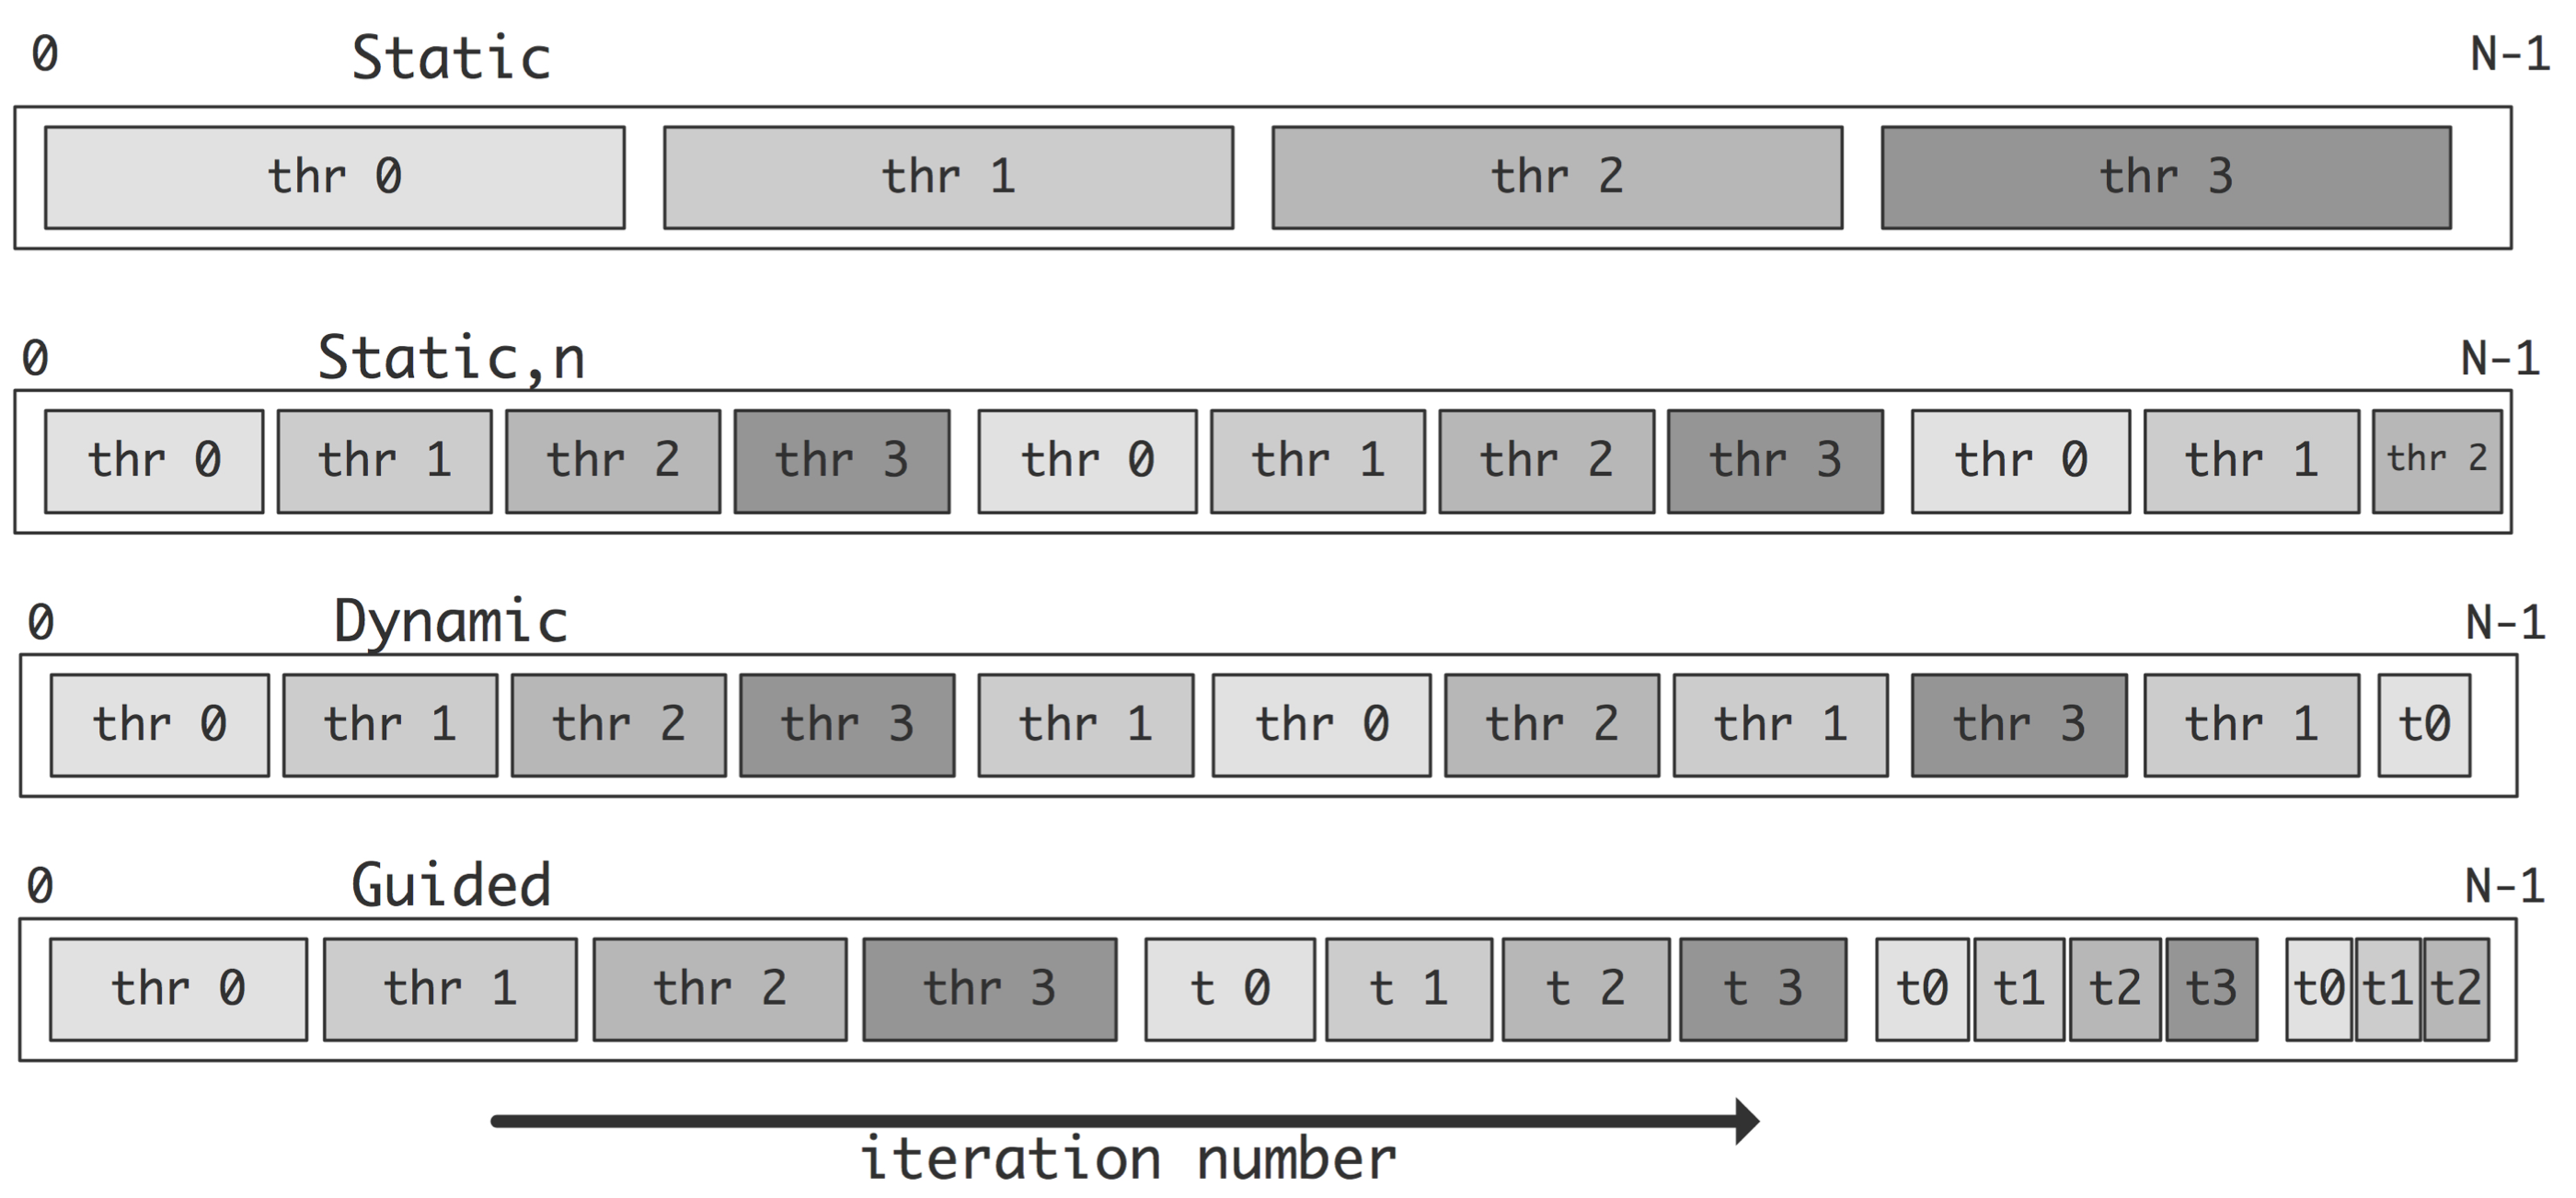
\includegraphics[width=1.0\textwidth]{Images/Loop_Schedule.png}
\caption{Illustration of the scheduling strategies of static, dynamic, and guided loop schedulers \cite{eijkhout_2021}.}
\label{Loop_Schedule}
\end{figure}

For this research project, we wish to look at parallelization of the 2D Advection Equation, 2D Inviscid Burgers' Equation, and 2D Viscous Burgers' Equation. In particular, we wish to look at strong and weak scaling, while incorporating cache blocking and loop scheduling. A detailed summary of our work can be found in Table \ref{Table_Timing_Summary}.


\begin{table}[t]
\begin{center}
\begin{tabular}{ |c|c|c|c|c|c| } 
\hline
 & Type of  & Scheduler & Number of x,y & Number of & Number of \\
 & Scaling  & Type & Steps ($N$) & Time Steps ($n$) &  Threads ($thrd\_cnt$) \\

\hline
\multirow{8}{4em}{2D Advection} & \multirow{4}{4em}{strong}& none & 32 - 2,048 & 10,000 & 1 - 8 \\ 
& & static & 32 - 2,048 & 10,000 & 1 - 8 \\
& & dynamic & 32 - 2,048 & 10,000 & 1 - 8 \\ 
&  & guided & 32 - 2,048 & 10,000 & 1 - 8 \\ 
& \multirow{4}{4em}{weak}& none & 32 - 2,048 & 1000$N$ $\div$ 32 & 1 - 8 \\ 
& & static & 32 - 2,048 & 1000$N$ $\div$ 32 & 1 - 8 \\
& & dynamic & 32 - 2,048 & 1000$N$ $\div$ 32 & 1 - 8 \\ 
&  & guided & 32 - 2,048 & 1000$N$ $\div$ 32 & 1 - 8 \\ 
\hline
\multirow{8}{4em}{2D Burgers} & \multirow{4}{4em}{strong}& none & 32 - 2,048 & 10,000 & 1 - 8 \\ 
& & static & 32 - 2,048 & 10,000 & 1 - 8 \\
& & dynamic & 32 - 2,048 & 10,000 & 1 - 8 \\ 
&  & guided & 32 - 2,048 & 10,000 & 1 - 8 \\ 
& \multirow{4}{4em}{weak}& none & 32 - 2,048 & 1000$N$ $\div$ 32 & 1 - 8 \\ 
& & static & 32 - 2,048 & 1000$N$ $\div$ 32 & 1 - 8 \\
& & dynamic & 32 - 2,048 & 1000$N$ $\div$ 32 & 1 - 8 \\ 
&  & guided & 32 - 2,048 & 1000$N$ $\div$ 32 & 1 - 8 \\ 
\hline
\multirow{8}{4em}{2D Viscous Burgers} & \multirow{4}{4em}{strong}& none & 32 - 2,048 & 10,000 & 1 - 8 \\ 
& & static & 32 - 2,048 & 10,000 & 1 - 8 \\
& & dynamic & 32 - 2,048 & 10,000 & 1 - 8 \\ 
&  & guided & 32 - 2,048 & 10,000 & 1 - 8 \\ 
& \multirow{4}{4em}{weak}& none & 32 - 2,048 & 1000$N$ $\div$ 32 & 1 - 8 \\ 
& & static & 32 - 2,048 & 1000$N$ $\div$ 32 & 1 - 8 \\
& & dynamic & 32 - 2,048 & 1000$N$ $\div$ 32 & 1 - 8 \\ 
&  & guided & 32 - 2,048 & 1000$N$ $\div$ 32 & 1 - 8 \\ 
\hline
\end{tabular}
\end{center}
\caption{Summary of tasks to run. Note that $N$ is only run for powers of 2.}
\label{Table_Timing_Summary}
\end{table}




\section{Results \& Discussion}

\subsection{Cache Blocking}

For the dynamic and static loop schedulers, we looked at the effect of chunk size on the time needed to run for the following setup: $N = 512$, $n = 10,000$, $thrd\_cnt = 8$, and the chunk size varied from a value of 1 up to a value of 100. The results are seen in Figure \ref{Chunk_Size}. Both static and dynamic scheduling have minimum times around a chunk size of 32 and 64. We believe the pattern displayed follows the formula

\begin{equation}
\ceil{\dfrac{N=512}{chunk\; size}} \div thrd\_cnt
\end{equation}

With a thread count of 8, this formula gives us integer values at local minima of 22, 32, and 64.This would follow a pattern such that at these minima every thread gets the same number of chunks, therefore all threads run at the same wall clock time. For other chunk sizes, some threads will carry more workload, some will carry less, thus producing uneven wall clock times and increasing overall computation time. 



\begin{figure}[h]
\centering
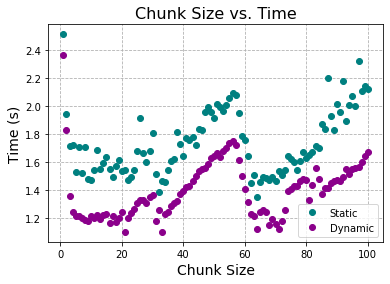
\includegraphics[width=1.0\textwidth]{Images/Chunk Size vs Time.png}
\caption{The effect of chunk size on computation time for schedule static and schedule dynamic.}
\label{Chunk_Size}
\end{figure}

\subsection{Loop Scheduling}

To investigate the effects that loop schedulers have on computation time, we looked at the effects of strong and weak scaling for a varying number of displacement steps, time steps, and thread count. For strong scaling, the time step was held constant at $n = 10,000$, while the thread count increased from $thrd\_cnt = 1$ through $thrd\_cnt = 8$, and the displacement steps increased by powers of 2 from $N = 32$ through $N = 2048$.

For weak scaling, the thread count increased from $thrd\_cnt$ = 1 through $thrd\_cnt = 8$, the displacement steps increased by powers of 2 from $N = 32$ through $N = 2048$, and the time step increased proportionally to $N$ by a factor of $1000/32$ for values of $n = 1000$ up to a value of $n = 64,000$. The results for all of these runs for 2D Advection, Inviscid Burgers, and Viscous Burgers can be found in Figures \ref{2D_Advection_Strong_Weak}, \ref{2D_Inviscid_Burgers_Strong_Weak}, and \ref{2D_Viscous_Burgers_Strong_Weak}.

Generally there is a trend that when you increase the number of threads, computation time decreases. Likewise, as the displacement mesh increases, the computation time increases. This trend is seen for both strong and weak scaling. However there are a few notable exceptions that we will outline below.

The first of these is that when the workload distributed to each thread is relatively small, the benefit of increasing thread count is overwhelmed by overhead. You can see this clearly in Figure ~\ref{2D_Advection_Strong_Weak}, especially in the runs without a scheduler and in the case of strong scaling, static advection. It is also fairly clear that this effect diminishes as the grid size increases, to the point where it is negligible in many runs, such as the guided runs.

The second major exception is found in the 2D weak scaling advection run in Figure \ref{2D_Advection_Strong_Weak}, specifically the one with no scheduler. The case of grid size $N =32$ appears to make sense to us. A major spike occurs when making the first thread, likely due to overhead in thread creation and memory management. This then decreases as you add threads up until 6, where it starts to reverse as threads are unable to find enough work to justify their creation. This, however, does not explain $N \in \{64, 128\}$ very well. Part of this is likely due to an interfering factor, as each doubling of $N$ will cause an eight-fold increase in workload (double the width, double the length, double the time steps). To some extent this is an open question. A similar trend can be seen in the Inviscid Burgers weak scaling run with a static scheduler (Figure \ref{2D_Inviscid_Burgers_Strong_Weak}).

\begin{figure}[p]
\vspace{-25mm}
\centering
\captionsetup[subfigure]{labelformat=empty}
\subfloat[]{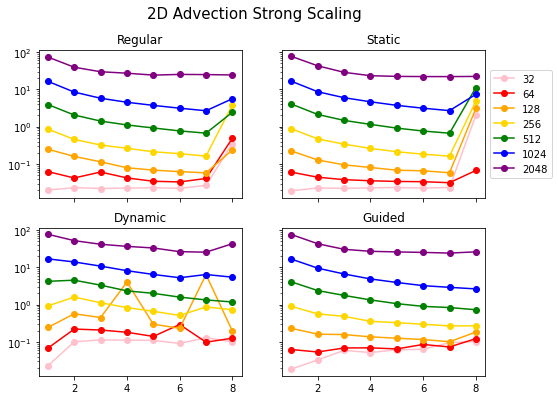
\includegraphics[width=14cm]{Images/2D_Advection_Strong_Scaling.png}}\\
\vfill
\subfloat[]{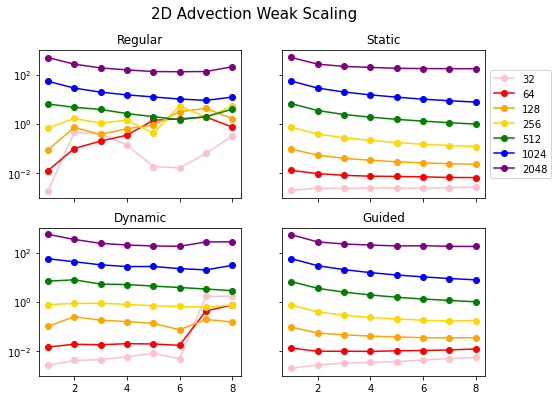
\includegraphics[width=14cm]{Images/2D_Advection_Weak_Scaling.png}}
\caption{Strong and weak scaling for the 2D Advection Equation} 
\label{2D_Advection_Strong_Weak}
\end{figure}

\begin{figure}[p]
\vspace{-25mm}
\centering
\captionsetup[subfigure]{labelformat=empty}
\subfloat[]{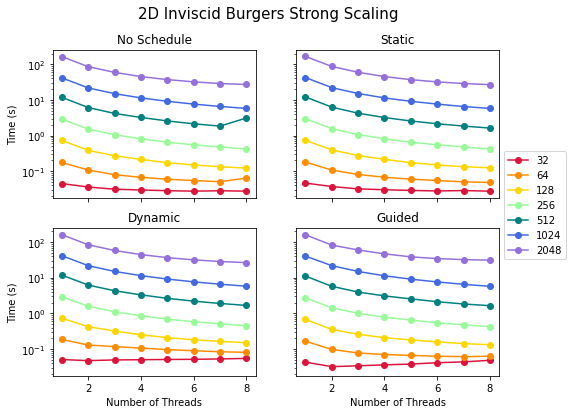
\includegraphics[width=14cm]{Images/2D_Inviscid_Burgers_Strong_Scaling.png}}\\
\vfill
\subfloat[]{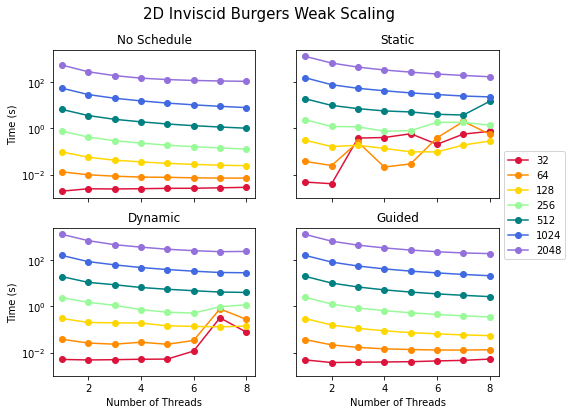
\includegraphics[width=14cm]{Images/2D_Inviscid_Burgers_Weak_Scaling.png}}
\caption{Strong and weak scaling for the 2D Inviscid Burgers' Equation} 
\label{2D_Inviscid_Burgers_Strong_Weak}
\end{figure}

\begin{figure}[p]
\vspace{-25mm}
\centering
\captionsetup[subfigure]{labelformat=empty}
\subfloat[]{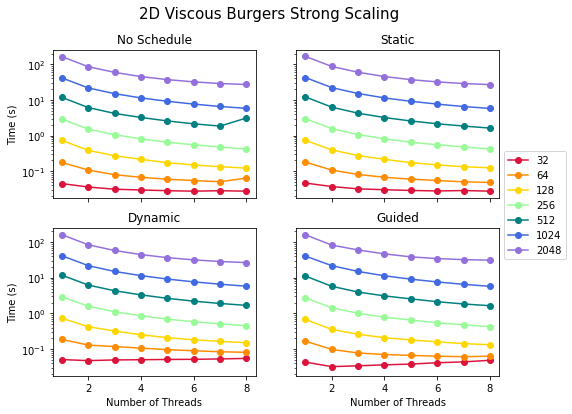
\includegraphics[width=14cm]{Images/2D_Viscous_Burgers_Strong_Scaling.png}}\\
\vfill
\subfloat[]{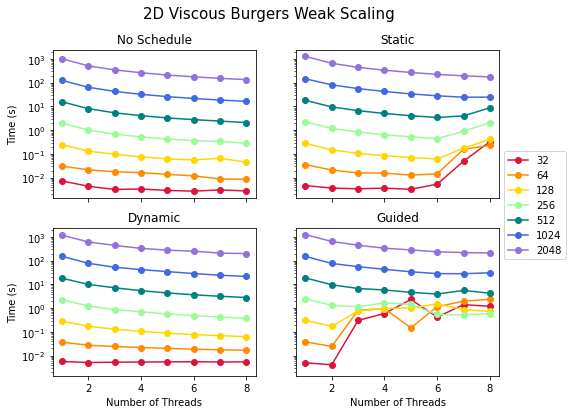
\includegraphics[width=14cm]{Images/2D_Viscous_Burgers_Weak_Scaling.png}}
\caption{Strong and weak scaling for the 2D Viscous Burgers' Equation} 
\label{2D_Viscous_Burgers_Strong_Weak}
\end{figure}

Figures \ref{2D_Advection_2048}, \ref{2D_Inviscid_Burgers_2048}, and \ref{2D_Viscous_Burgers_2048} show a detailed comparison of strong and weak scaling for various loop schedulers. These comparisons correspond to the $N = 2,048$ cases shown previously for the 2D Advection, Inviscid Burgers', and Viscous Burgers' Equations.

For the 2D Advection Equation shown in Figure \ref{2D_Advection_2048}, run time is minimized with no scheduler with $\sim$6-7 threads. The static scheduler works better for strong scaling, but only slightly, whereas no scheduler performs faster for weak scaling.

For the 2D Inviscid and Viscous Burgers' Equations shown in Figures \ref{2D_Inviscid_Burgers_2048} and \ref{2D_Viscous_Burgers_2048}, no scheduler is clearly best for the case of weak scaling. There is also little-to-no variation between the other schedulers in terms of strong scaling. For all four cases, there is a general trend of increasing the thread count decreasing the computation time. 

The overarching question of this research project is ``How can I make my code run faster?'' To that, we answer, more threads, no scheduler.

\begin{figure}[p]
\centering
\captionsetup[subfigure]{labelformat=empty}
\subfloat[]{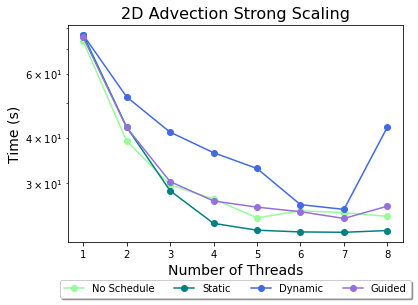
\includegraphics[width=12cm]{Images/2D_Advection_Strong_N_2048.png}}\\
\vfill
\subfloat[]{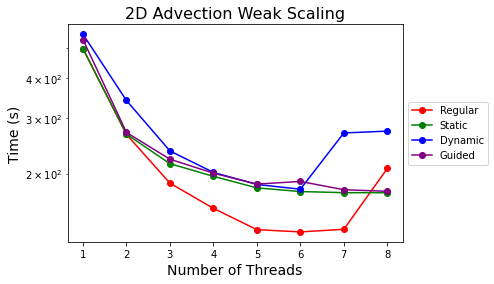
\includegraphics[width=12cm]{Images/2D_Advection_Weak_N_2048.png}}
\caption{2D Advection Equation} 
\label{2D_Advection_2048}
\end{figure}

\begin{figure}[p]
\centering
\captionsetup[subfigure]{labelformat=empty}
\subfloat[]{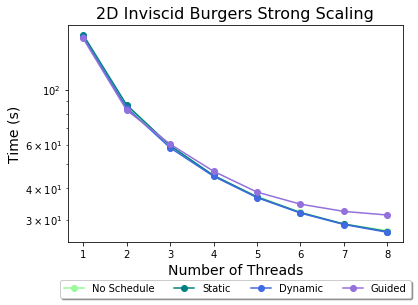
\includegraphics[width=12cm]{Images/2D_Inviscid_Burgers_Strong_N_2048.png}}\\
\vfill
\subfloat[]{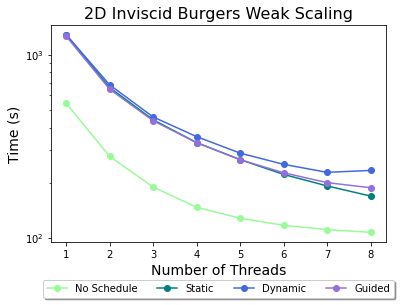
\includegraphics[width=12cm]{Images/2D_Inviscid_Burgers_Weak_N_2048.png}}
\caption{2D Inviscid Burgers' Equation} 
\label{2D_Inviscid_Burgers_2048}
\end{figure}

\begin{figure}[p]
\centering
\captionsetup[subfigure]{labelformat=empty}
\subfloat[]{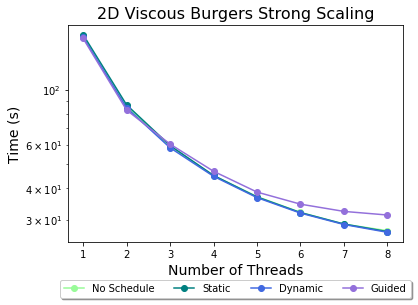
\includegraphics[width=12cm]{Images/2D_Viscous_Burgers_Strong_N_2048.png}}\\
\vfill
\subfloat[]{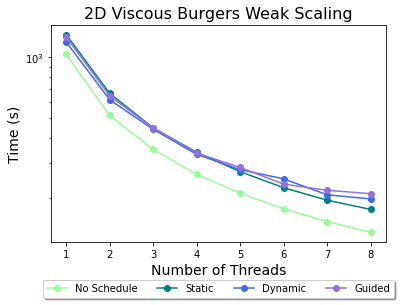
\includegraphics[width=12cm]{Images/2D_Viscous_Burgers_Weak_N_2048.png}}
\caption{2D Viscous Burgers' Equation} 
\label{2D_Viscous_Burgers_2048}
\end{figure}

\section{Acknowledgments}

C. W. would like to thank Dr. Andrew Christlieb for his invaluable knowledge on numerical solutions to hyperbolic PDEs. C. W. and G. A. would both like to thank Dr. Bill Punch for teaching us how to run our code faster.







 \bibliography{Final_Report_Bibliography} 
\bibliographystyle{apalike}

\end{document}